

\documentclass[a4paper,11pt]{article}

\usepackage[T1]{fontenc}
\usepackage[utf8]{inputenc}
\usepackage{graphicx}
\usepackage{xcolor}

\renewcommand\familydefault{\sfdefault}
\usepackage{tgheros}

\usepackage{amsmath,amssymb,amsthm,textcomp}
\usepackage{enumerate}
\usepackage{multicol}
\usepackage{tikz}
\usepackage{CJKutf8}

\usepackage{geometry}
\geometry{left=25mm,right=25mm,%
bindingoffset=0mm, top=20mm,bottom=20mm}


\linespread{1.3}

\newcommand{\linia}{\rule{\linewidth}{0.5pt}}
% my own titles
\makeatletter
\renewcommand{\maketitle}{
\begin{center}
\vspace{2ex}
{\huge \textsc{\@title}}
\vspace{1ex}
\\
\linia\\
\@author \hfill \@date
\vspace{4ex}
\end{center}
}
\makeatother
%%%


%%%----------%%%----------%%%----------%%%----------%%%

\begin{document}

\title{Assignment 1}


\author{
\begin{CJK*}{UTF8}{gbsn}
Name: 林柏均
\end{CJK*}
Student ID: s107062240}

\date{03/22/2021}

\maketitle

\section{Part 1}
\subsection{Read in and print out all the data fields in a DICOM file}

\begin{figure}[h]
\centering
\includegraphics[width=0.5\textwidth]{Figure1.png}
\caption{The metadata of a particular slice image}
\label{fig1}
\end{figure}

\subsection{Read in the raw data for a CT slice and convert its pixel values into Hounsfield units. Compute the max, min, mean and standard deviation of both images.}

\begin{table}[h]
\centering
\caption{Max, Min, Mean and Standard Deviation of both images} \label{tab1}
\begin{tabular}{|l|l|l|}
\hline
Property &  Raw Data & Hounsfiled Units\\
\hline
Max &  {\bfseries\centering 2415} & {\bfseries\centering 1391}\\
Min &  {\bfseries\centering -2000} & {\bfseries\centering -3024}\\
Mean &  {\bfseries\centering 157.39} & {\bfseries\centering -866.61}\\
Standard Deviation &  {\bfseries\centering 1175.97} & {\bfseries\centering 1175.97}\\
\hline
\end{tabular}
\end{table}
\pagebreak

\section{Part 2}

\subsection{Sort all the slices to make it into correct order}
Since we know that the metadata of the slice image including the SliceLocation, therefore, we can easily sort the Location and then get the sorted set of slice images.

\subsection{Normalize all the pixel from Hounsfield Units to float32 type number between 0.0 to 1.0 and display 25 slices in correct order}

We know that the minimum value of the original image is -1024, and we need to convert it to 0-base, therefore, I add 1024 for entire image and than divide the whole image by 4096 so that the value can be set between 0 and 1. \\

Figure 2 shows that one of the patient slices with sorted order, and it presents after setting as Hounsfield Units to float32 type.


\begin{figure}[h]
\centering
\includegraphics[width=0.5\textwidth]{25slices.png}
\caption{Above figure show 25 slices with sorted order after setting as Hounsfield Units}
\label{fig1}
\end{figure}

\pagebreak

\section{Part 3}

\subsection{Try to use at least two different thresholding algorithm to segment the lung}

1. Mean Threshold
We calculate the mean value of the image using np.mean(image), if the pixel value greate or equal to the mean value, then we set the pixel value as 1, otherwise, we set the pixel value as 0. (Result shown as Figure 3) 

\begin{figure}[h]
\centering
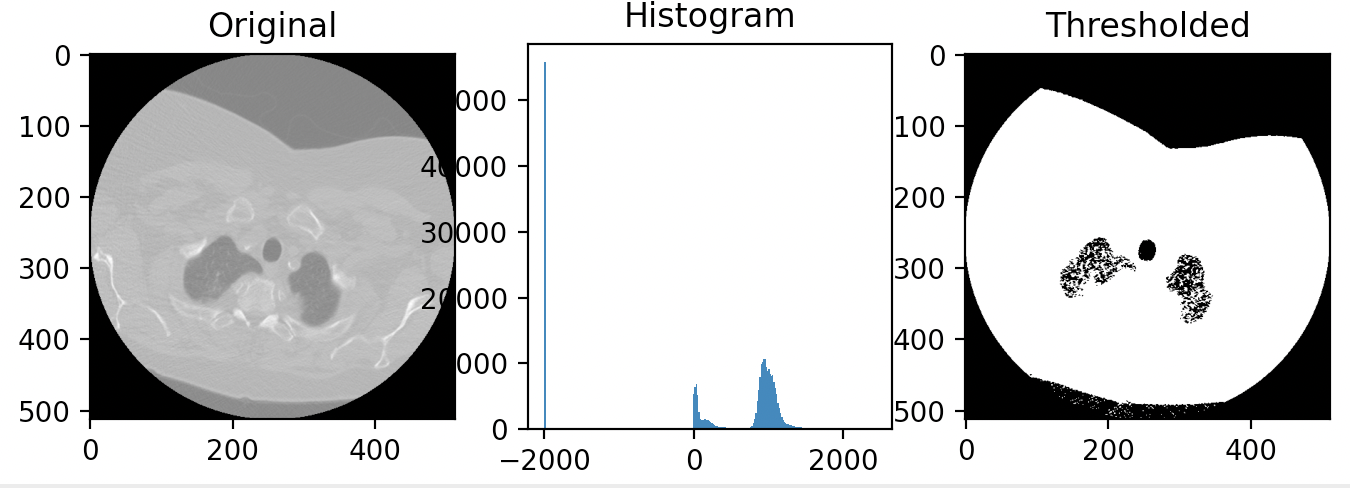
\includegraphics[width=0.8\textwidth]{mean.png}
\caption{Above figure show 25 slices with sorted order after setting as Hounsfield Units}
\label{fig1}
\end{figure}

2. Medium Threshold
We calculate the mean value of the image using np.median(image), if the pixel value greate or equal to the median value, then we set the pixel value as 1, otherwise, we set the pixel value as 0. (Result shown as Figure 3) 

\begin{figure}[h]
\centering
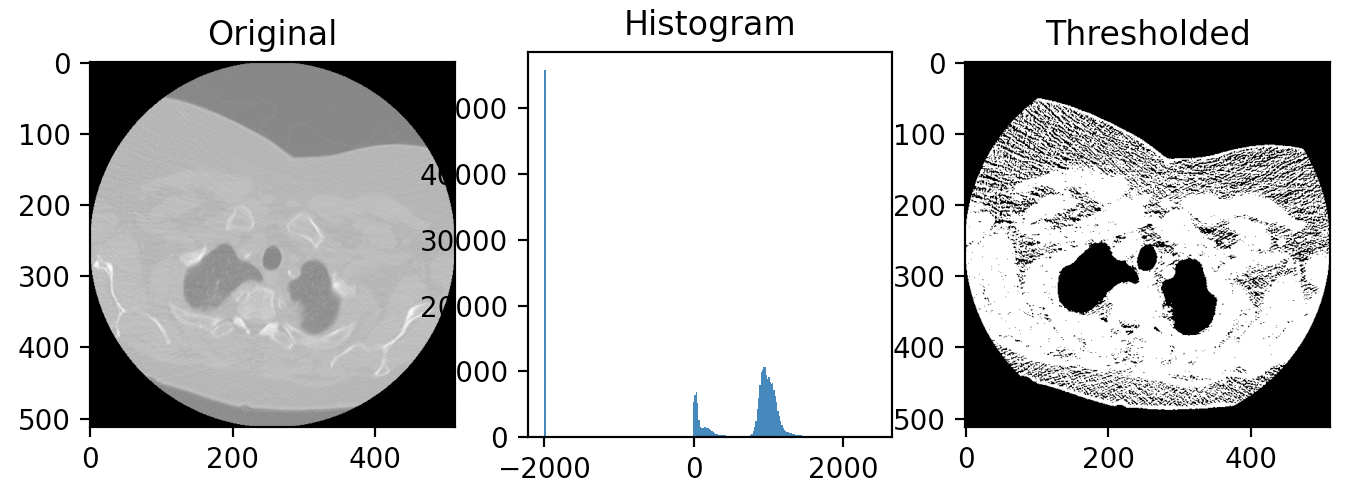
\includegraphics[width=0.8\textwidth]{medium.png}
\caption{Above figure show 25 slices with sorted order after setting as Hounsfield Units}
\label{fig1}
\end{figure}

\pagebreak

\section{Question and Summary}

Computed Tomography is quite a unfamiliar domain for me, therefore, it spent a lot of time for me to understand the CT image and how to manipulate them. \\

In Part 1, I learned that every .DICOM file will store lots of information of the slice, and we can use this information to do some stuff, including sorting the slices and so forth. \\ 

In Part 2, according to the metadata of the slice, we can find the correct sorted order of the slices, furthermore, if we find out the sorted order, then we can create the corresponding 3D module. \\

In Part 3, thresholding algorithm can help us emphasize the important part or the unclear part in the original image. In this assignment, I implenmented two basice thresholding algorithm, mean and medium. 


\end{document}
